\documentclass[12pt,a4paper]{article}
\usepackage[utf8]{inputenc}
\usepackage[pdfauthor={Luciano Henrique de Oliveira Santos}]{hyperref}
\usepackage[right=2.5cm,left=2.5cm,top=2cm,bottom=2cm]{geometry}
\usepackage{url}
\usepackage{graphicx}
\usepackage{float}
\usepackage{setspace}
\usepackage[export]{adjustbox}

\renewcommand{\familydefault}{\sfdefault}

\title{Clue in Prolog\\{\Large -- A Didactic Example --}}
\author{Luciano Santos}
\date{August 2016}

\begin{document}

\maketitle

\section{Introduction}

This is the documentation for a simple script in SWI-Prolog that plays the game Clue\footnote{\url{http://www.hasbro.com/en-us/toys-games/hasbro-games:clue} (accessed on August, 2016)}. This implementation follows a didactic approach, not aimed at creating an advanced AI system that employs complex strategies and human behaviour models to master the game. It simply illustrates how a declarative language can be used to play a relatively simple game based on a certain set of rules.

The implementation is based on the rules for the 2002 version of the game (see PDF on the root folder) and the board on Figure \ref{fig:board}.

\begin{figure}[H]
	\centering
	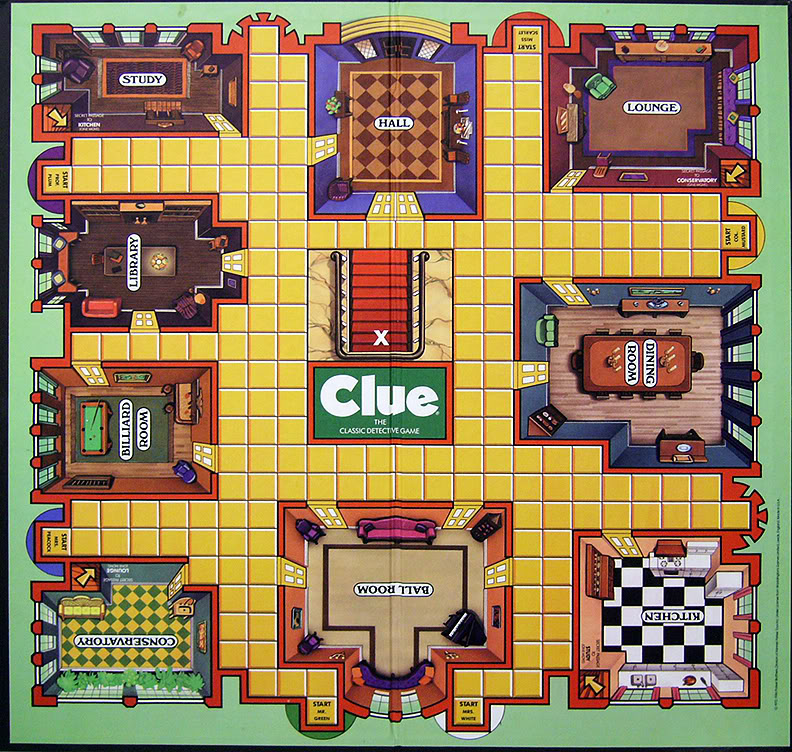
\includegraphics[width=0.5\textwidth]{board.jpg}
	\caption{The game board.}
	\label{fig:board}
\end{figure}

The following principles were observed in this implementation to make it simple:
\begin{itemize}
    \item no long-term planning -- for each action and information received, the agent updates its 'knowledge base' and, on each turn, it makes an independent decision based on the current knowledge, instead of following a planned route;
    
    \item no lucky guesses -- the agent only makes an accusation if it's certain that it's true;
    
    \item no poker face -- the agent only acts to acquire more information, and will not make a move or guess for the sole purpose of misleading other players;
    
    \item no mind reading -- the agent will not infer information from other players actions, except facts that can be logically proven; it will not try to predict how people would or should behave, however, it will assume that everyone will play strategically, \textit{e.g.}, if the player to the left has already shown a certain card before, that card will not be used on a next guess, because a smart player would keep showing the same card over and over again, even if she had a different one to show.
\end{itemize}

The sections below describe the rationale and the details of this implementation. Section \ref{sec:board} explains how the game board and the current position of each player is stored internally and how the agent finds the shortest path to a given goal. Section \ref{sec:data} describes how the knowledge acquired as the match progresses is represented, and how the game decides which action to take on each turn. Finally, Section \ref{sec:interface} brings the predicates that allow the final user to start a new game and interact with the agent.

\section{The Board}
\label{sec:board}

\section{The Data}
\label{sec:data}

\section{The Interface}
\label{sec:interface}

\end{document}
